% This is samplepaper.tex, a sample chapter demonstrating the
% LLNCS macro package for Springer Computer Science proceedings;
% Version 2.20 of 2017/10/04
%
\documentclass[tikz,runningheads,a4paper]{llncs}
%
\usepackage[portuges]{babel}
\usepackage[utf8x]{inputenc}

\usepackage{graphicx}
% Used for displaying a sample figure. If possible, figure files should
% be included in EPS format.
%
% If you use the hyperref package, please uncomment the following line
% to display URLs in blue roman font according to Springer's eBook style:
% \renewcommand\UrlFont{\color{blue}\rmfamily}

%% Useful packages
\usepackage[font=small,labelfont=bf]{caption} % Required for specifying captions to tables and figures

\graphicspath{ {./Images/} }
\usepackage[colorlinks=False]{hyperref} % add links inside PDF files
\usepackage{amsmath}  % Math fonts
\usepackage{amsfonts} %
\usepackage{amssymb}  %
\usepackage{multirow}
\usepackage{float}
\usepackage{cite}
\usepackage{tikz-cd} 

\begin{document}
%
\title{CLAV - ESPECIFICAÇÃO E VERIFICAÇÃO DO MODELO FORMAL}
%
%\titlerunning{Abbreviated paper title}
% If the paper title is too long for the running head, you can set
% an abbreviated paper title here
%
\author{Armando Santos \and
Gonçalo Duarte}

%
\authorrunning{A. et al.}
% First names are abbreviated in the running head.
% If there are more than two authors, 'et al.' is used.
%
\institute{University of Minho, Braga, Portugal}
%
\maketitle              % typeset the header of the contribution
%
\begin{abstract}

CLAV é uma plataforma que está a ser desenvolvida pelo Departamento de Informática da Universidade do Minho em parceria com a Direção Geral do Livro, Arquivos e Bibliotecas (DGLAB), e tem como objetivo a classificação e avaliação de todos os documentos que circulam pelas instituições públicas portuguesas. Neste momento existe um modelo do problema especificado em OWL (\textit{Ontology Web Language}), mas tem sofrido várias alterações no decorrer do último ano e não existiu tempo para estudar o impacto dessas mesmas alterações nas pré-condições e invariantes do modelo. Neste projeto, inserido na Unidade Curricular de Laboratórios em Engenharia Informática (LEI) do MIEI/UM, pretende-se formalizar o modelo de raíz assim como os seus invariantes e garantir a consistência dos mesmos, sendo capaz de detetar erros que, até agora, não tenham sido identificados.

\keywords{Administração Pública \and Métodos Formais \and Engenharia Informática \and Alloy Analyzer \and OWL.}
\end{abstract}
%
%
%
\section{Introdução}

Até agora, em Portugal, não existia nenhum sistema de informação que gerisse a classificação e a avaliação dos documentos gerados no âmbito dos processos que circulam dentro das instituições públicas portuguesas. O CLAV veio mudar isso com a elaboração de um catálogo, que se pretende que venha a ser a referência nacional de todos processos da Administração Pública (AP), tendo sido modelado numa ontologia. Esta ontologia está especificada num modelo formal que representa o conjunto de conceitos referentes aos processos de negócio e aos relacionamentos entre eles. Infelizmente, todos os dados e documentação de apoio estão espalhados, desorganizados e em diferentes formatos, o que os torna extremamente difíceis de manter num domínio tão complexo como o da AP. No entanto, embora já tenham sido feitos esforços para criar um formato neutro, como a Macro-estrutura Funcional (MEF), e vários sistemas de exploração e exportação, devido aos problemas associados com a inserção manual dos dados oriundos das diversas instituições e à complexidade e instabilidade dos invariantes e restrições associadas ao modelo não é possível garantir a coerência das relações entre os processos de negócio. Esta incoerência é extremamente crítica uma vez que a classificação e avaliação dos processos possuí legislações associadas e lida com a remoção ou conservação (digital e física) de documentos governamentais\cite{clav-new}.

Deste modo, no contexto da unidade curricular de Laboratórios em Engenharia Informática do Mestrado Integrado em Engenharia Informática da Universidade do Minho e associado ao perfil de Métodos Formais em Engenharia Informática, apresentamos, neste artigo, a especificação e verificação, de raíz, da ontologia e o estudo da coerência dos invariantes e pré-condições que fazem parte dela. Devido à natureza puramente relacional inerente no domínio do problema em questão, iremos tirar partido de métodos algébricos e relacionais para nos ajudar a raciocinar sobre o problema em mãos e utilizar o Alloy \textit{model checker} para nos auxiliar a encontrar falhas no desenho do modelo.

\section{O Problema}

\begin{figure}[H]
\centering
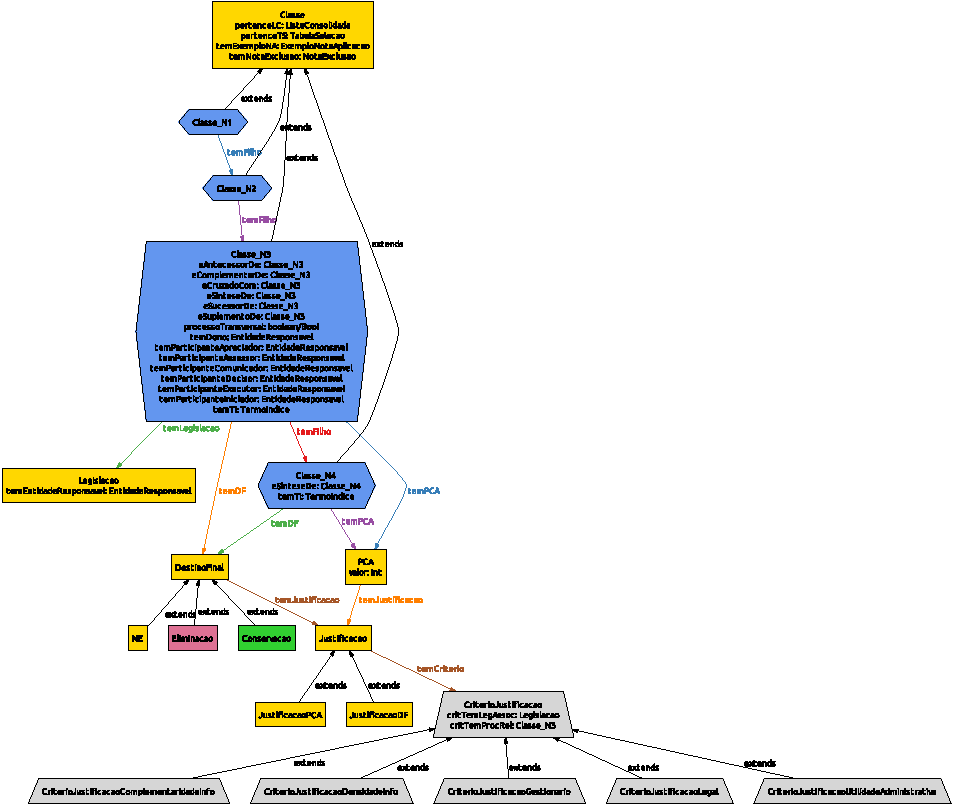
\includegraphics[width=\linewidth]{metamodel.pdf}
\caption{Meta-modelo simplificado}
\label{metamodel}
\end{figure}

Cada instituição pública portuguesa desempenha uma função específica dentro da AP (p. ex. a prestação de cuidados de saúde), associado a cada função existe um conjunto de várias sub-funções (p. ex. a gestão de utentes e serviços clínicos) e cada sub-função possui uma lista de processos de negócio que, concretamente, se materializam em documentos (p. ex. um processo de negócio pertencente à sub-função de gestão de utentes seria o registo clínico de utentes). A Lista Consolidada (LC) possui esta estrutura hierárquica de 4 níveis\cite{clav-mod} onde os processos de negócio são passíveis de ser desdobrados para efeitos de avaliação. Cada classe da LC possui um conjunto de atributos que a descreve e a partir do 3º nível (PNs) começam a surgir relações mais complicadas entre processos no campo chamado contexto de avaliação. Este contexto de avaliação, como também iremos ver mais à frente, tem associado um conjunto de invariantes que influenciarão o campo das decisões de avaliação. Este último campo é responsável por conter a informação sobre o Prazo de Conservação Administrativa (PCA) e Destino Final (DF) de um processo que correspondem, respetivamente, ao prazo que o documento deve ser guardado e qual o seu destino uma vez que este prazo expire.

Embora as entidades principais no domínio do problema sejam as classes da LC, existem várias outras que se relacionam direta ou indiretamente com cada uma das classes e que fornecem uma maior profundidade e complexidade ao modelo como podemos observar na figura \ref{metamodel}.

Observando o meta-modelo simplificado, onde a azul se encontram os 4 nivéis de classe, verificamos que este possui uma complexidade natural mesmo sem lhe impor alguma restrição. Sendo assim, e dado o contexto sério em que o problema está inserido, torna-se claro que deve ser feita alguma coisa no que diz respeito a dar algumas garantias acerca da coerência e consistência da LC.

\subsection{Primeiro \textit{Checkpoint}}

Sendo o CLAV um projeto que já existe há 1 ano e já se encontra com alguns componentes operacionais, decidiu-se pegar em toda a documentação existente sobre o modelo e os seus requisitos e, com a ajuda do Professor José Carlos Ramalho, fazer um apanhado de todas as entidades e relações existentes. Durante esta primeira fase, bastantes das reuniões semanais serviram para apurar pequenos detalhes e dúvidas que iam surgindo.

Uma das razões que motivaram este investimento inicial, apesar de já existir uma ontologia definida pela qual nos podíamos guiar, foi a de existir muita documentação\cite{clav-new}\cite{clav-mod}\cite{clav-req} solta e incompleta que nem sempre estava de acordo com a versão mais recente da ontologia. Foi então, elaborado um documento, atualizado, que documenta os mais recentes requisitos e invariantes e que já se tornou bastante útil no refinamento da ontologia original, nomeadamente na eliminação de entidades e relações obsoletas e no apuramento do domínio e contradomínio de várias relações.

Na Secção \ref{SecModel} iremos falar mais detalhadamente sobre cada entidade e relação do modelo e na secção \ref{SecAlloy} será abordada a respetiva implementação em Alloy.

\subsection{Segundo \textit{Checkpoint}}

Uma das principais motivações deste projeto é estudar a forma como os mais variados invariantes interagem entre si e se, de alguma forma, se contradizem. É neste sentido que o Alloy, sendo uma linguagem de modelação de software leve que nos permite especificar tanto o modelo como as restrições a ele associadas, ajuda a detetar erros ingénuos e subtis.

Após o investimento inicial em colecionar todo o material relevante e necessário sobre o problema, deu-se início ao ciclo de vida de verificação do problema \cite{jno}. Apesar dos invariantes serem abordados com mais detalhes na secção \ref{SubSecInv}, é possível adiantar já que foram identificadas 38 restrições no total, sendo que 23 dessas foram acrescentadas no tal processo de verificação.

Podemos então concluir, que o Alloy teve um impacto positivo na análise das restrições do modelo e na especificação do modelo formal. É importante realçar que a utilização de um \textit{model checker} não descarta a necessidade de prova mas é muito útil para encontrar falhas de \textit{design} como pudemos constatar. A ausência de contra-exemplos dá uma grande confiança de que uma prova de correção está ao alcance.

\subsection{Avaliação Final}

\section{Modelo Formal} \label{SecModel}

Nesta secção será abordada a especificação formal do CLAV. Será introduzida alguma notação relativa ao cálculo relacional utilizado na formalização do problema e, posteriormente, tanto as classes presentes no domínio do modelo como as relações entre estas serão enunciadas. Por último, devido à grande quantidade de invariantes existentes, apenas serão apresentados X, que melhor ilustram a dimensão e complexidade do CLAV. % TODO: mudar X para um número concreto.

\subsection{Calcular com relações\cite{jno}\cite{jno-5}}

Dentro do contexto do CLAV podemos encontrar frases do género \textit{"A gestão de utentes é uma subfunção da prestação de cuidados de saúde"}, \textit{"O processo de referenciação de utentes para consultas é cruzado com o processo de registo nacional de utentes"} ou \textit{"Se um processo é complementar de outro, então o seu destino final é de conservação"}. Estas expressões podem ser interpretadas como relações tipadas entre objetos.

As relações, como as frases a cima, já existem na matemática há vários anos e possuem uma notação própria capaz de as exprimir. Em geral, a notação (infixa) \textit{b R a}, onde \textit{a} e \textit{b} são os objetos e \textit{R} a relação, é a que expressa mais naturalmente as relações. Esta notação aplica-se também ao uso da voz passiva, que expressa a relação inversa de \textit{R}, denotada por \textit{Rº}, onde \textit{b R a} significa o mesmo que \textit{a Rº b}. Por exemplo, \textit{é síntese deº = é sintetizado por}.

Também é importante observar que relações do género \textit{R = é o pai de}, são relações em que quando conhecido, o pai (p. ex. de uma classe) é único. Relações com esta propriedade são referidas como \textit{simples} e satisfazem a propriedade

\begin{equation}
\label{eq-simple}
R \circ Rº \subseteq id
\end{equation}

\noindent onde ($\circ$), denota a composição de relações, \textit{id} é a relação identidade e $\subseteq$ é a inclusão de relações:

\begin{equation}
\label{eq-subseteq}
R \subseteq S \equiv \forall b; a : b R a \Rightarrow b S a.
\end{equation}

\subsubsection{Relações tipadas e diagramas:}

O uso de setas e diagramas torna possível expressar formulas relacionais mais complexas. No entanto, para ser possível representar e raciocinar sobre estes diagramas é necessário que estes estejam bem construídos.

Observando a relação \eqref{eq-subseteq} concluímos que apenas faz sentido se \textit{R} e \textit{S} forem do mesmo tipo. A notação $B \xleftarrow[]{\text{R}} A$ declara uma relação binária que relaciona \textit{B's} com \textit{A's}. Por exemplo, B = \textit{Classe nível 1} e A = \textit{Classe nível 2} para o caso em que \textit{R = é o pai de}. 

Caminhos em diagramas são construídos a partir do encadeamento de setas, o que corresponde à composição de relações:

\begin{equation}
\label{eq-composition}
\begin{tikzcd}
A \arrow[bend right, leftarrow, swap]{rr}{R\ \circ\ S} \arrow[leftarrow]{r}{R} & B \arrow[leftarrow]{r}{S} & C
\end{tikzcd}
\hskip2cm b (R \circ S) a \equiv \exists a: b R a \land a S c
\end{equation}

Os diagramas também advêm da comparação de caminhos, por exemplo,

\begin{center}
\begin{tikzcd}[row sep=tiny]
Classe\_N2 \arrow[swap]{dd}{temFilho12} &           & ListaConsolidada \arrow[swap]{ll}{pertenceLC2} \arrow{dd}{id} \\
                                      & \subseteq &                                                       \\
Classe\_N1                      &           & ListaConsolidada \arrow{ll}{pertenceLC1}  
\end{tikzcd}
\end{center}

\noindent que representa a restrição

\begin{equation}
\label{eq-inv1}
    temFilho12 \circ pertenceLC2 \subseteq id \circ pertenceLC1,
\end{equation}

\noindent onde, no domínio do CLAV, as relações simples \textit{pertenceLC1} e \textit{pertenceLC2} mapeiam, respetivamente, cada classe de nível 1 na sua respetiva LC e cada classe de nível 2 na sua respetiva LC, a relação simples, \textit{temFilho12}, relaciona uma classe de nível 1 com os seus filhos (classes de nível 2), a relação \textit{id} é a conhecida relação identidade que relaciona cada objeto consigo próprio.

\subsubsection{Dos diagramas à lógica\cite{jno}\cite{jno-5}:}

O que é que a expressão \eqref{eq-inv1} significa em lógica proposicional?

\begin{equation*}
    temFilho12 \circ pertenceLC2 \subseteq id \circ pertenceLC1
\end{equation*}
$\equiv$ \{ inclusão de relações \eqref{eq-subseteq}; id \}
\begin{equation*}
    \forall\ c1, lc : c1\ (temFilho12 \circ pertenceLC2)\ lc \Rightarrow c1\ pertenceLC2\ lc
\end{equation*}
$\equiv$ \{ composição (3) \}
\begin{equation*}
    \forall\ c1, lc : (\exists\ c2 : c1\ temFilho12\ c2\ \land\ c2\ pertenceLC2\ lc) \Rightarrow c1\ pertenceLC1\ lc
\end{equation*}
$\equiv$ \{ \textit{splitting; nesting} \}
\begin{equation*}
    \forall\ c1, c2, lc : c2\ pertenceLC2\ lc \land c1\ temFilho12\ c2\ \Rightarrow \ c1\ pertenceLC1\ lc
\end{equation*}

\noindent Literalmente:
\vskip0.2cm
\textit{Se uma c2 pertence à lista consolidada lc e c2 é filho da classe c1, então c1 também pertence à lista consolidada lc.}

\vskip0.2cm
\noindent Ainda em menos palavras, a restrição \eqref{eq-inv1}, sugere:
\vskip0.2cm
\textit{Filho de quem pertence, também pertence.}

\subsection{Domínio}

%Introduzir cada uma das signatures e o seu contexto no problema.

\subsection{Relações envolvidas}

%Falar nas relações em geral e em especifico as mais importantes envolvidas na classificação e avaliação de PNs

\subsection{Invariantes} \label{SubSecInv}

%Formalizar o modelo e os seus invariantes

\section{Modelação em ALLOY} \label{SecAlloy}

\subsection{Especificação}

%Fazer a ponte entre o modelo formal e o modelo Alloy

\subsection{Verificação}

%Pendente.

\section{Dificuldades}

%Documentação do projeto do CLAV:
%    - espalhada
%    - desorganizada
%    - desatualizada
%    Implicações:
%        - Tivemos que fazer o apanhado de tudo

%Alguns dos invariantes não eram estáveis e sofreram alterações ao longo do projeto assim como alguns pormenores relacionados com o modelo em si.

\section{Conclusão e Trabalho Futuro} \label{SecConclusion}

%
% ---- Bibliography ----
%
% BibTeX users should specify bibliography style 'splncs04'.
% References will then be sorted and formatted in the correct style.
%
% \bibliographystyle{splncs04}
% \bibliography{mybibliography}
%
\bibliographystyle{splncs04}
\bibliography{mybib}{}

\end{document}
